\documentclass[]{article}
\usepackage{lmodern}
\usepackage{amssymb,amsmath}
\usepackage{ifxetex,ifluatex}
\usepackage{fixltx2e} % provides \textsubscript
\ifnum 0\ifxetex 1\fi\ifluatex 1\fi=0 % if pdftex
  \usepackage[T1]{fontenc}
  \usepackage[utf8]{inputenc}
\else % if luatex or xelatex
  \ifxetex
    \usepackage{mathspec}
  \else
    \usepackage{fontspec}
  \fi
  \defaultfontfeatures{Ligatures=TeX,Scale=MatchLowercase}
\fi
% use upquote if available, for straight quotes in verbatim environments
\IfFileExists{upquote.sty}{\usepackage{upquote}}{}
% use microtype if available
\IfFileExists{microtype.sty}{%
\usepackage{microtype}
\UseMicrotypeSet[protrusion]{basicmath} % disable protrusion for tt fonts
}{}
\usepackage[margin=1in]{geometry}
\usepackage{hyperref}
\hypersetup{unicode=true,
            pdftitle={Statistical Inference Part2},
            pdfauthor={Sandesh},
            pdfborder={0 0 0},
            breaklinks=true}
\urlstyle{same}  % don't use monospace font for urls
\usepackage{color}
\usepackage{fancyvrb}
\newcommand{\VerbBar}{|}
\newcommand{\VERB}{\Verb[commandchars=\\\{\}]}
\DefineVerbatimEnvironment{Highlighting}{Verbatim}{commandchars=\\\{\}}
% Add ',fontsize=\small' for more characters per line
\usepackage{framed}
\definecolor{shadecolor}{RGB}{248,248,248}
\newenvironment{Shaded}{\begin{snugshade}}{\end{snugshade}}
\newcommand{\AlertTok}[1]{\textcolor[rgb]{0.94,0.16,0.16}{#1}}
\newcommand{\AnnotationTok}[1]{\textcolor[rgb]{0.56,0.35,0.01}{\textbf{\textit{#1}}}}
\newcommand{\AttributeTok}[1]{\textcolor[rgb]{0.77,0.63,0.00}{#1}}
\newcommand{\BaseNTok}[1]{\textcolor[rgb]{0.00,0.00,0.81}{#1}}
\newcommand{\BuiltInTok}[1]{#1}
\newcommand{\CharTok}[1]{\textcolor[rgb]{0.31,0.60,0.02}{#1}}
\newcommand{\CommentTok}[1]{\textcolor[rgb]{0.56,0.35,0.01}{\textit{#1}}}
\newcommand{\CommentVarTok}[1]{\textcolor[rgb]{0.56,0.35,0.01}{\textbf{\textit{#1}}}}
\newcommand{\ConstantTok}[1]{\textcolor[rgb]{0.00,0.00,0.00}{#1}}
\newcommand{\ControlFlowTok}[1]{\textcolor[rgb]{0.13,0.29,0.53}{\textbf{#1}}}
\newcommand{\DataTypeTok}[1]{\textcolor[rgb]{0.13,0.29,0.53}{#1}}
\newcommand{\DecValTok}[1]{\textcolor[rgb]{0.00,0.00,0.81}{#1}}
\newcommand{\DocumentationTok}[1]{\textcolor[rgb]{0.56,0.35,0.01}{\textbf{\textit{#1}}}}
\newcommand{\ErrorTok}[1]{\textcolor[rgb]{0.64,0.00,0.00}{\textbf{#1}}}
\newcommand{\ExtensionTok}[1]{#1}
\newcommand{\FloatTok}[1]{\textcolor[rgb]{0.00,0.00,0.81}{#1}}
\newcommand{\FunctionTok}[1]{\textcolor[rgb]{0.00,0.00,0.00}{#1}}
\newcommand{\ImportTok}[1]{#1}
\newcommand{\InformationTok}[1]{\textcolor[rgb]{0.56,0.35,0.01}{\textbf{\textit{#1}}}}
\newcommand{\KeywordTok}[1]{\textcolor[rgb]{0.13,0.29,0.53}{\textbf{#1}}}
\newcommand{\NormalTok}[1]{#1}
\newcommand{\OperatorTok}[1]{\textcolor[rgb]{0.81,0.36,0.00}{\textbf{#1}}}
\newcommand{\OtherTok}[1]{\textcolor[rgb]{0.56,0.35,0.01}{#1}}
\newcommand{\PreprocessorTok}[1]{\textcolor[rgb]{0.56,0.35,0.01}{\textit{#1}}}
\newcommand{\RegionMarkerTok}[1]{#1}
\newcommand{\SpecialCharTok}[1]{\textcolor[rgb]{0.00,0.00,0.00}{#1}}
\newcommand{\SpecialStringTok}[1]{\textcolor[rgb]{0.31,0.60,0.02}{#1}}
\newcommand{\StringTok}[1]{\textcolor[rgb]{0.31,0.60,0.02}{#1}}
\newcommand{\VariableTok}[1]{\textcolor[rgb]{0.00,0.00,0.00}{#1}}
\newcommand{\VerbatimStringTok}[1]{\textcolor[rgb]{0.31,0.60,0.02}{#1}}
\newcommand{\WarningTok}[1]{\textcolor[rgb]{0.56,0.35,0.01}{\textbf{\textit{#1}}}}
\usepackage{graphicx,grffile}
\makeatletter
\def\maxwidth{\ifdim\Gin@nat@width>\linewidth\linewidth\else\Gin@nat@width\fi}
\def\maxheight{\ifdim\Gin@nat@height>\textheight\textheight\else\Gin@nat@height\fi}
\makeatother
% Scale images if necessary, so that they will not overflow the page
% margins by default, and it is still possible to overwrite the defaults
% using explicit options in \includegraphics[width, height, ...]{}
\setkeys{Gin}{width=\maxwidth,height=\maxheight,keepaspectratio}
\IfFileExists{parskip.sty}{%
\usepackage{parskip}
}{% else
\setlength{\parindent}{0pt}
\setlength{\parskip}{6pt plus 2pt minus 1pt}
}
\setlength{\emergencystretch}{3em}  % prevent overfull lines
\providecommand{\tightlist}{%
  \setlength{\itemsep}{0pt}\setlength{\parskip}{0pt}}
\setcounter{secnumdepth}{0}
% Redefines (sub)paragraphs to behave more like sections
\ifx\paragraph\undefined\else
\let\oldparagraph\paragraph
\renewcommand{\paragraph}[1]{\oldparagraph{#1}\mbox{}}
\fi
\ifx\subparagraph\undefined\else
\let\oldsubparagraph\subparagraph
\renewcommand{\subparagraph}[1]{\oldsubparagraph{#1}\mbox{}}
\fi

%%% Use protect on footnotes to avoid problems with footnotes in titles
\let\rmarkdownfootnote\footnote%
\def\footnote{\protect\rmarkdownfootnote}

%%% Change title format to be more compact
\usepackage{titling}

% Create subtitle command for use in maketitle
\providecommand{\subtitle}[1]{
  \posttitle{
    \begin{center}\large#1\end{center}
    }
}

\setlength{\droptitle}{-2em}

  \title{Statistical Inference Part2}
    \pretitle{\vspace{\droptitle}\centering\huge}
  \posttitle{\par}
    \author{Sandesh}
    \preauthor{\centering\large\emph}
  \postauthor{\par}
      \predate{\centering\large\emph}
  \postdate{\par}
    \date{10/23/2019}


\begin{document}
\maketitle

\hypertarget{were-going-to-analyze-the-toothgrowth-data-in-the-r-datasets-package.}{%
\subsection{We're going to analyze the ToothGrowth data in the R
datasets
package.}\label{were-going-to-analyze-the-toothgrowth-data-in-the-r-datasets-package.}}

\hypertarget{load-the-toothgrowth-data-and-perform-some-basic-exploratory-data-analyses}{%
\subsection{1. Load the ToothGrowth data and perform some basic
exploratory data
analyses}\label{load-the-toothgrowth-data-and-perform-some-basic-exploratory-data-analyses}}

We plot the lengt vs the dose for each of the supplements. To gain a
better view of groth rates, we also add a loess curve. We see that the
growth rates seem to behave differently for both supplements.

\begin{Shaded}
\begin{Highlighting}[]
\KeywordTok{library}\NormalTok{(ggplot2)}
\KeywordTok{data}\NormalTok{(ToothGrowth)}
\KeywordTok{qplot}\NormalTok{(dose, len, }\DataTypeTok{data=}\NormalTok{ToothGrowth, }\DataTypeTok{facets=}\NormalTok{.}\OperatorTok{~}\NormalTok{supp, }\DataTypeTok{geom=}\KeywordTok{c}\NormalTok{(}\StringTok{"point"}\NormalTok{, }\StringTok{"smooth"}\NormalTok{), }\DataTypeTok{method=}\StringTok{"loess"}\NormalTok{)}
\end{Highlighting}
\end{Shaded}

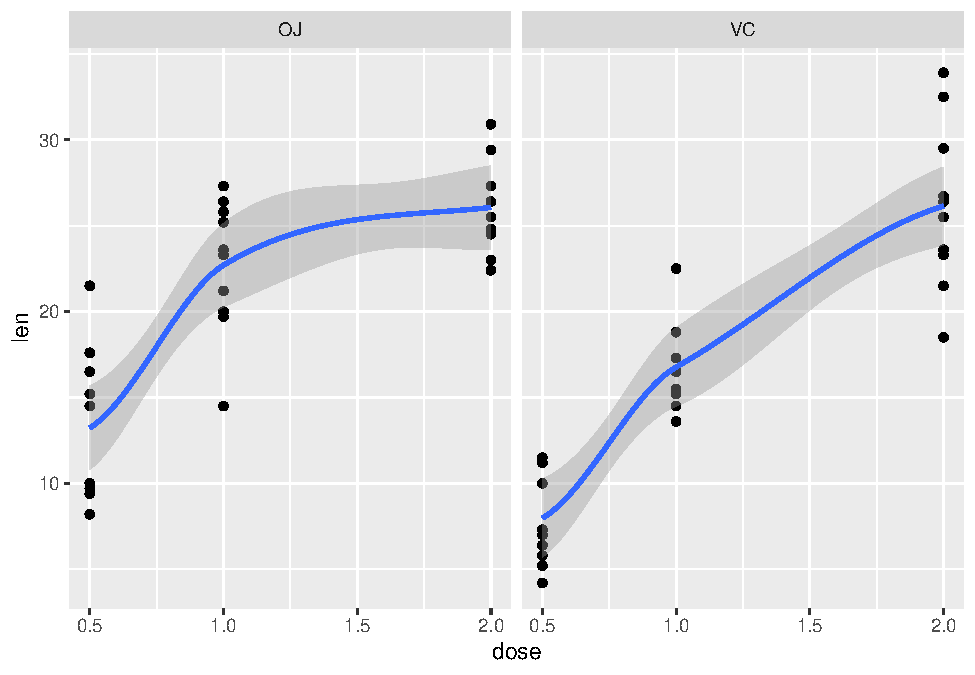
\includegraphics{Part2_files/figure-latex/unnamed-chunk-1-1.pdf} \#\# 2.
Provide a basic summary of the data.

This dataset contains three variables: supplement, dose and len. For
each supplement, and each dose we calculate basic descriptive
statistics: standard deviation, variance, and mean.

\begin{Shaded}
\begin{Highlighting}[]
\NormalTok{dose <-}\StringTok{ }\KeywordTok{as.numeric}\NormalTok{(}\KeywordTok{levels}\NormalTok{(}\KeywordTok{as.factor}\NormalTok{(ToothGrowth}\OperatorTok{$}\NormalTok{dose)))}
\NormalTok{supp <-}\StringTok{ }\KeywordTok{levels}\NormalTok{(ToothGrowth}\OperatorTok{$}\NormalTok{supp)}
\CommentTok{# Structured for further processing}
\NormalTok{data <-}\StringTok{ }\KeywordTok{list}\NormalTok{()}
\NormalTok{x <-}\StringTok{ }\KeywordTok{Map}\NormalTok{(}\ControlFlowTok{function}\NormalTok{(s) \{}
  \KeywordTok{Map}\NormalTok{(}\ControlFlowTok{function}\NormalTok{(d) \{}
\NormalTok{    l <-}\StringTok{ }\NormalTok{ToothGrowth}\OperatorTok{$}\NormalTok{len[ToothGrowth}\OperatorTok{$}\NormalTok{dose }\OperatorTok{==}\StringTok{ }\NormalTok{d }\OperatorTok{&}\StringTok{ }\NormalTok{ToothGrowth}\OperatorTok{$}\NormalTok{supp }\OperatorTok{==}\StringTok{ }\NormalTok{s]}
\NormalTok{    data <<-}\StringTok{ }\KeywordTok{rbind}\NormalTok{(data, }\KeywordTok{list}\NormalTok{(}\DataTypeTok{supp =}\NormalTok{ s, }\DataTypeTok{dose =}\NormalTok{ d, }\DataTypeTok{sd=}\KeywordTok{sd}\NormalTok{(l), }\DataTypeTok{var=}\KeywordTok{var}\NormalTok{(l), }\DataTypeTok{mu=}\KeywordTok{mean}\NormalTok{(l)))}
\NormalTok{  \}, dose)}
\NormalTok{\}, supp)}
\NormalTok{data}
\end{Highlighting}
\end{Shaded}

\begin{verbatim}
##      supp dose sd       var      mu   
## [1,] "OJ" 0.5  4.459709 19.889   13.23
## [2,] "OJ" 1    3.910953 15.29556 22.7 
## [3,] "OJ" 2    2.655058 7.049333 26.06
## [4,] "VC" 0.5  2.746634 7.544    7.98 
## [5,] "VC" 1    2.515309 6.326778 16.77
## [6,] "VC" 2    4.797731 23.01822 26.14
\end{verbatim}

\hypertarget{use-confidence-intervals-and-hypothesis-tests-to-compare-tooth-growth-by-supp-and-dose.-use-the-techniques-from-class-even-if-theres-other-approaches-worth-considering}{%
\subsection{3. Use confidence intervals and hypothesis tests to compare
tooth growth by supp and dose. (Use the techniques from class even if
there's other approaches worth
considering)}\label{use-confidence-intervals-and-hypothesis-tests-to-compare-tooth-growth-by-supp-and-dose.-use-the-techniques-from-class-even-if-theres-other-approaches-worth-considering}}

We perform the student-t test for each dose level between the two
supplements:

\begin{Shaded}
\begin{Highlighting}[]
\NormalTok{tests =}\StringTok{ }\KeywordTok{list}\NormalTok{()}
\ControlFlowTok{for}\NormalTok{ (d }\ControlFlowTok{in}\NormalTok{ dose) \{}
\NormalTok{  ojd <-}\StringTok{ }\NormalTok{ToothGrowth}\OperatorTok{$}\NormalTok{len[ToothGrowth}\OperatorTok{$}\NormalTok{dose }\OperatorTok{==}\StringTok{ }\NormalTok{d }\OperatorTok{&}\StringTok{ }\NormalTok{ToothGrowth}\OperatorTok{$}\NormalTok{supp }\OperatorTok{==}\StringTok{ "OJ"}\NormalTok{]}
\NormalTok{  vcd <-}\StringTok{ }\NormalTok{ToothGrowth}\OperatorTok{$}\NormalTok{len[ToothGrowth}\OperatorTok{$}\NormalTok{dose }\OperatorTok{==}\StringTok{ }\NormalTok{d }\OperatorTok{&}\StringTok{ }\NormalTok{ToothGrowth}\OperatorTok{$}\NormalTok{supp }\OperatorTok{==}\StringTok{ "VC"}\NormalTok{]}
\NormalTok{  t <-}\StringTok{ }\KeywordTok{t.test}\NormalTok{(ojd, vcd, }\DataTypeTok{var.equal=}\NormalTok{T)}
\NormalTok{  id <-}\StringTok{ }\KeywordTok{paste}\NormalTok{(}\StringTok{"OJ"}\NormalTok{, d, }\StringTok{"-"}\NormalTok{, }\StringTok{"VC"}\NormalTok{, d)}
\NormalTok{  tests <-}\StringTok{ }\KeywordTok{rbind}\NormalTok{(tests, }\KeywordTok{list}\NormalTok{(}\DataTypeTok{id=}\NormalTok{id, }\DataTypeTok{p.value=}\NormalTok{t}\OperatorTok{$}\NormalTok{p.value, }\DataTypeTok{ci.lo=}\NormalTok{t}\OperatorTok{$}\NormalTok{conf.int[}\DecValTok{1}\NormalTok{], }\DataTypeTok{ci.hi=}\NormalTok{t}\OperatorTok{$}\NormalTok{conf.int[}\DecValTok{2}\NormalTok{]))}
\NormalTok{\}}
\NormalTok{tests}
\end{Highlighting}
\end{Shaded}

\begin{verbatim}
##      id                p.value      ci.lo     ci.hi   
## [1,] "OJ 0.5 - VC 0.5" 0.005303661  1.770262  8.729738
## [2,] "OJ 1 - VC 1"     0.0007807262 2.840692  9.019308
## [3,] "OJ 2 - VC 2"     0.9637098    -3.722999 3.562999
\end{verbatim}

\hypertarget{state-your-conclusions-and-the-assumptions-needed-for-your-conclusions.}{%
\subsection{4. State your conclusions and the assumptions needed for
your
conclusions.}\label{state-your-conclusions-and-the-assumptions-needed-for-your-conclusions.}}

First, we assume that variance in all groups should be expected to be
equal. The underlying assumption is that sampling of Guinea Pigs to
assign them to a supplement and a dose was done properly.

Based on the test results from the previous question we need to
\textbf{reject} the following hypotheses:

\begin{itemize}
\tightlist
\item
  True difference in means between OJ 0.5 and VC 0.5 is equal to 0
\item
  True difference in means between OJ 1 and VC 1 is equal to 0
\item
  True difference in means between OJ 2 and VC 2 is equal to 0
\end{itemize}


\end{document}
